\documentclass{standalone}
\usepackage{tikz}
\begin{document}
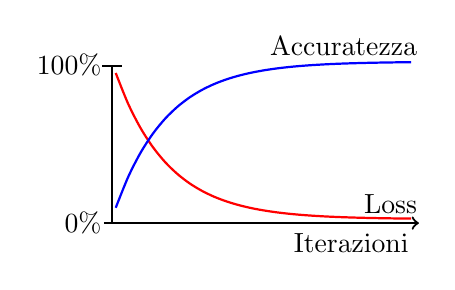
\begin{tikzpicture}
    \draw[thick, ->](-0.1,0)--++(4,0)node[below left]{Iterazioni};
    \draw[-|, thick](0,0)node[left]{$0\%$}--++(0,2.01)node[left]{$100\%$};
    \draw[thick, red]plot[smooth, domain=0.05:3.8](\x, {2*e^(-\x*1.5)+0.05});
    \draw[thick, blue]plot[smooth, domain=0.05:3.8](\x, {2-2*e^(-\x*1.5)+0.05});
    \draw(4,0)node[above left]{Loss};
    \draw(4,2)node[above left]{Accuratezza};
\end{tikzpicture}
\end{document}